\documentclass[UTF8]{ctexart}
\usepackage{amsmath}
\usepackage{float}
\usepackage{indentfirst}
\usepackage{listings}
\usepackage{xcolor}
\lstset{
    %backgroundcolor=\color{red!50!green!50!blue!50},%代码块背景色为浅灰色
    rulesepcolor= \color{gray}, %代码块边框颜色
    breaklines=true,  %代码过长则换行
    numbers=left, %行号在左侧显示
    numberstyle= \small,%行号字体
    %keywordstyle= \color{red},%关键字颜色
    %commentstyle=\color{green!90}, %注释颜色
    frame=shadowbox%用方框框住代码块
    }
\usepackage{graphicx}
\usepackage[a4paper, left = 3.17cm, right = 3.17cm, top=2.54cm, bottom=2.54cm]{geometry}
\setlength{\parindent}{2em}
\title{第七讲-习题}
\author{姜帆}
\date{\today}
\begin{document}
\maketitle
\tableofcontents
\newpage
\section{vins代码仿真数据接口修改}
\indent 在test文件夹中新$simulation.cpp$作为运行仿真数据的函数接口。主要重写
$PubImuData()、PubImageData()$函数。IMU数据按照仿真生成数据格式读取便可,图像数据由于仿真生成的是
每帧图像所得到的固定的36个特征点,因此读入特征点的像素坐标,并导入系统中,生成对应的$feature_buf$即可,不需要进行
匹配跟踪。\\
\begin{figure}[H]
\centering
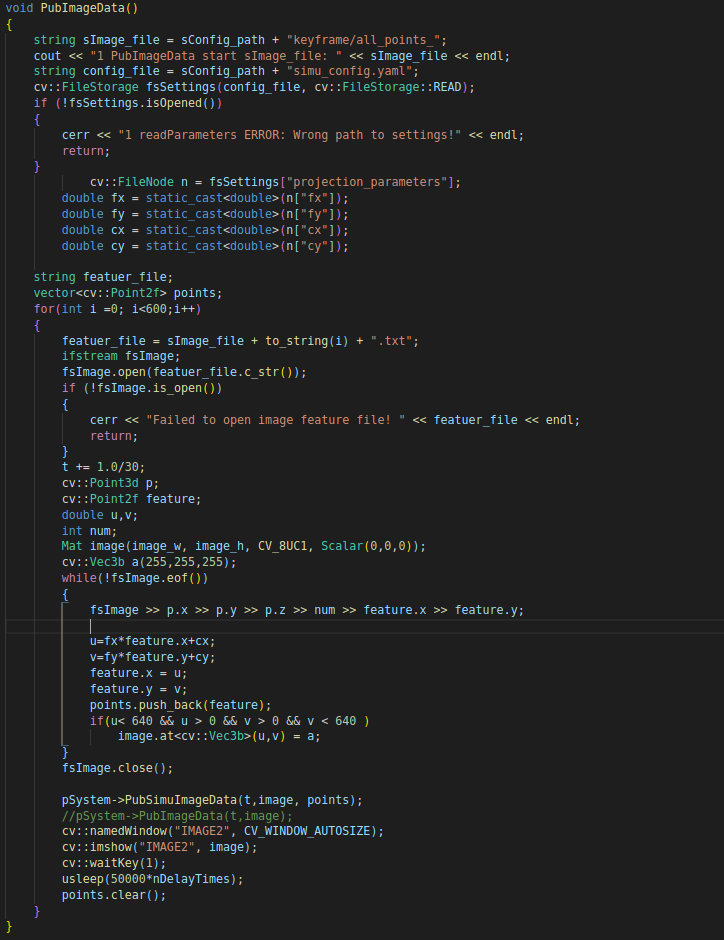
\includegraphics[width=0.8\textwidth]{1.png}    
\caption{代码修改}
\label{img0}
\end{figure}
\indent 跟踪模块作出如下修改,直接对特征点进行赋值,不需要对图像进行角点提取与光流跟踪。\\
\begin{figure}[H]
\centering
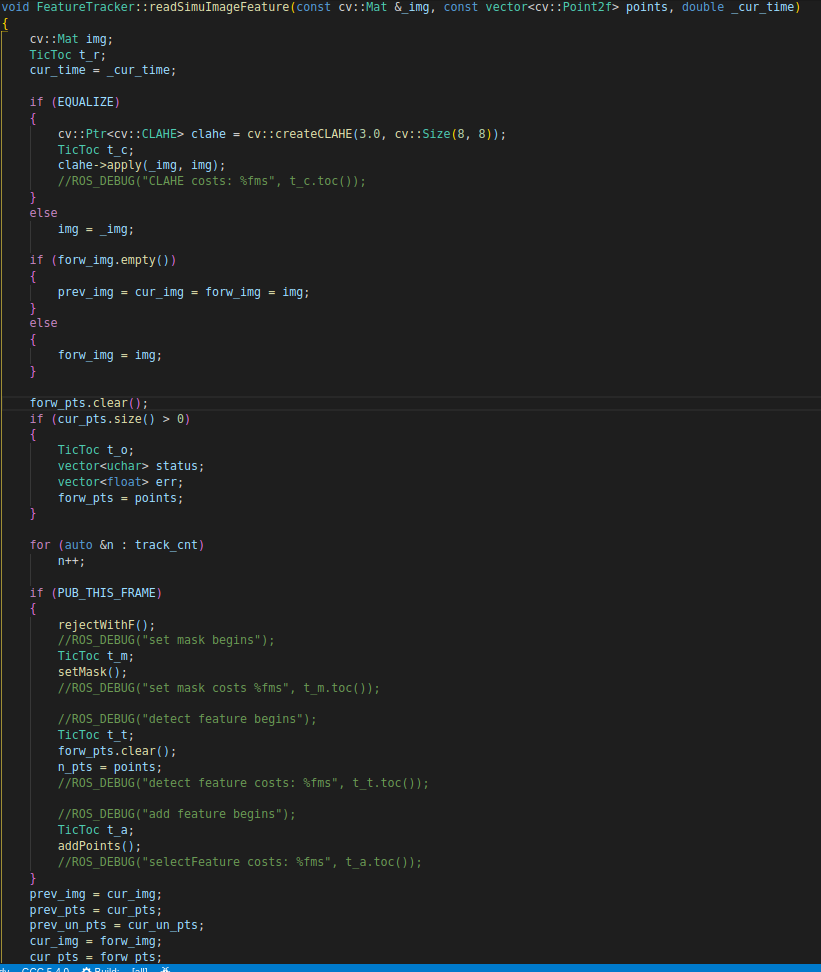
\includegraphics[width=0.8\textwidth]{2.png}    
\caption{代码修改}
\label{img0}
\end{figure}
% \section{无噪声仿真数据实验}
% \section{加噪声仿真数据实验}
\end{document}